\documentclass[12pt,a4paper]{article}

% ---------- Page layout ----------
\usepackage[a4paper,margin=2.5cm]{geometry}
\usepackage{setspace}
\onehalfspacing
\setlength{\parindent}{0pt}
\setlength{\parskip}{0.75em}

% ---------- Tables and figures ----------
\usepackage{graphicx}
\usepackage{booktabs}
\usepackage{threeparttable}
\usepackage{caption}
\usepackage{float}
\usepackage{array}
\usepackage{tabularx}
\usepackage{eurosym}

% ---------- Math and symbols ----------
\usepackage{amsmath}
\usepackage{amssymb}

% ---------- References ----------
\usepackage[round,authoryear]{natbib}
\bibliographystyle{apalike}

% ---------- Links ----------
\usepackage{xcolor}
\usepackage[colorlinks=true,linkcolor=black,citecolor=blue,urlcolor=blue]{hyperref}

% ---------- Thesis metadata ----------
\newcommand{\thesistitle}{Whose Perception of Geopolitical Risk Is Priced in Defence Equities?\\[0.4em]Evidence from the Russia--Ukraine War}
\newcommand{\thesisauthor}{Khrystyna Kateryna Valenia}
\newcommand{\thesisdate}{August 2026}

\begin{document}

%--------------------------------------------------------------
\begin{titlepage}
  \centering
  \vspace*{2cm}
  {\LARGE\thesistitle\par}
  \vspace{1cm}
  {\large \thesisauthor\par}
  \vspace{0.5cm}
  {\large \thesisdate\par}
  \vspace{1cm}
  \begin{abstract}
  \noindent
  Every standard measure of geopolitical risk is built from English-language newspapers. This thesis asks whether that editorial vantage point is the one that matters for defence-equity prices, or whether local-language perception --- from Ukrainian and Russian outlets, closer to the conflict --- carries additional information. Using 4,027 days of multilingual news data from GDELT's translingual archive, classified by the publisher's national identity rather than by article subject, this thesis tests whether Ukrainian, Russian state, and Russian independent coverage of the Russia--Ukraine war explains defence-equity returns conditional on Western coverage already being in the regression. The answer is no. Local perception adds nothing in coverage volume, in tone, or in the structure of anticipatory versus realised reporting, across two asset classes (defence equities and European natural gas) and one non-market outcome (realised escalation). A power simulation on 1,855 out-of-sample days confirms the test would detect an effect of 0.5\% out-of-sample R$^2$ with 82\% power: the range the literature treats as economically meaningful is ruled out. Russian state media's tone did not move when Russia invaded Ukraine ($+0.02$); Ukrainian media's tone fell by 1.66 points. Markets track one of those two signals.
  \end{abstract}
\end{titlepage}

\newpage
\tableofcontents
\newpage

%==============================================================
\section{Introduction}
%==============================================================

The Russia--Ukraine war is the most intensively covered armed conflict in modern media history, and it produced the sharpest repricing of defence equities in decades. Defence indices rose 20--30\% in the weeks around the February 2022 invasion and have continued to respond to developments in the conflict since. For an investor trying to understand that repricing, the natural question is: what information is driving it? The standard answer in the geopolitical-risk literature is ``what newspapers say'' --- but which newspapers? The two most widely used indices, those of \citet{caldara2022} and \citet{baker2016}, are built from a fixed panel of English-language, mostly American and British outlets. When a defence-equity price is said to be responding to geopolitical risk, it is responding to a quantity constructed from one particular editorial perspective --- the Western one.

\textbf{The research question of this thesis is: whose perception of geopolitical risk is priced in defence equities?} Two candidate answers are possible. Either the information that moves defence-equity prices originates where the war is fought --- in Ukrainian and Russian media, which are closer to the battlefield, cover it more intensively, and carry it earlier --- and reaches Western prices with the delay that translation and attention impose. Or Western markets price the Western narrative, and local coverage, however earlier or more voluminous, adds nothing once the Western signal is controlled for.

\textbf{The first challenge is measurement.} The submitted version of this project built Ukrainian, Russian, and Western sentiment series from GDELT's Global Knowledge Graph version 1.0 --- a stream that is effectively English-only (7 articles from \texttt{.ru} domains out of 60,690 in a typical day), in which nationality was assigned by the country an article \textit{mentioned}, not by the country that published it. The series labelled Ukrainian and Russian sentiment were, in practice, English-language articles about Ukraine and Russia: one population sorted by topic and relabelled as three perspectives. This makes the source-group comparison meaningless. The correction is to use GDELT's \textit{translingual} archive, which processes material in 65 source languages and classifies each article by the outlet that published it, providing genuine Ukrainian and Russian media signals. The rebuilt indices run from 18 February 2015, when the translingual archive begins, and cover 4,027 calendar days.

\textbf{The second challenge is identification.} News coverage of a conflict and defence-equity prices may move together for many reasons that have nothing to do with the media ecosystem carrying the signal. Both respond to the same underlying events; financial market conditions affect both; and a common regime trend contaminates any level regression. The strategy addresses this through a conditional joint F-test: local media are asked whether they add to returns \textit{conditional on Western coverage already being in the regression}. This mirrors the test in \citet{bondarenko2024}: they ask whether local Russian risk measures add to English-language measures for the Russian economy; this thesis asks the same question for the counterparty's assets. Because the correct market control for European defence equities is a European index (not the S\&P 500, which was used in the submitted version), the analysis uses STOXX 600 returns as the market control, which eliminates an artefactual result documented in Section~\ref{sec:robustness}.

\textbf{The third challenge is multiple testing.} The specification grid crosses frequency (daily, weekly), episode window (six anticipation periods plus the full sample), and five defence-equity targets, producing 31 testable cells. Running 31 tests at 5\% significance would yield roughly 1.5 false rejections by chance. The analysis applies Benjamini--Hochberg correction across the full grid and, for the anticipation-structure test (Gate 3), pre-registers the pass rule, the excluded targets, and the sign condition before building the test. Gates 4 and 5 each have their data ingested after the pre-registration is written. This sequence is verifiable from repository commit history.

\textbf{The fourth challenge is evaluating a null result.} A finding that nothing predicts is worthless unless the reader knows what could have been found. The out-of-sample section of this thesis therefore accompanies its zero Clark--West rejections with a power simulation: using the actual return series and implanting a predictor with a known true effect, the design is shown to detect an out-of-sample R$^2$ of 0.5\% with 82\% power and 1.0\% with 98\% power on 1,855 out-of-sample days. The range of effect sizes the predictability literature treats as economically meaningful is therefore ruled out.

\textbf{The main findings are threefold.} First, local-language perception adds nothing to defence-equity returns conditional on Western coverage, across four tests, two asset classes, and one non-market outcome. The positive control --- the Western block tested in the same cells --- is detected in 2--3 of 31 cells in each gate, confirming the design has power to find effects where they exist. Second, the descriptive evidence reveals a striking asymmetry: Russian state media's conflict tone did not move when Russia invaded Ukraine (aggregate shift: $+0.02$; fixed-outlet panel of 24 state outlets: $-0.05$), while Ukrainian media's tone fell by 1.66 points on the same scale. This asymmetry is both the most interesting empirical fact in the data and consistent with the null finding about pricing: the information set that changed most sharply at the invasion is not the one that markets track. Third, across 50 out-of-sample forecasting specifications, the Clark--West test rejects zero times against 2.5 expected by chance, and simulation confirms this is not a power failure.

\textbf{These findings speak to three literatures.} The primary contribution is to the literature on whose information is priced in financial markets. \citet{bondarenko2024} show that for the Russian domestic economy, local Russian-language risk perception matters and English-language perception does not. This thesis runs the mirror test on the counterparty's assets and finds the reverse: Western defence equities price the Western narrative, and the local narrative is redundant. Neither result says ``local media always matter'' or ``local media never matter''; together they say that each market prices the information ecosystem it inhabits, which is a more specific and more useful claim. Second, this thesis contributes to the text-based risk measurement literature. Since \citet{baker2016} and \citet{caldara2022} established newspaper counts as a workable risk proxy, the question of which newspapers has been underexplored. \citet{tetlock2007media} shows that negative media content predicts short-run market movements, and \citet{manela2017} link news-implied volatility to disaster risk over more than a century of data. \citet{loughran2011textual} caution that automated sentiment dictionaries require domain-specific validation, which is why GDELT tone in this thesis is interpreted as an indicator of negativity rather than a direct measure of investor beliefs. A previous project that measured Ukrainian and Russian sentiment from an English-only stream --- effectively measuring the topic of articles rather than their provenance --- illustrates exactly why the question matters: the measurement error is not small. Third, this thesis contributes to the defence-equity literature. Studies such as \citet{apergis2018defense}, \citet{zhang2022race}, \citet{covachev2024europe}, and \citet{klomp2025hamas} show that defence equities respond to geopolitical events around armed conflicts, but they aggregate all news rather than separating national source groups. This thesis shows that the response is driven by the Western narrative layer, not by the local-language one that is closer to the events in question.

%==============================================================
\section{Data and Identification Strategy}
\label{sec:data}
%==============================================================

\subsection{The news corpus and its construction}

The analysis rests on a corpus of 4,027 days of conflict-related news from GDELT's Translingual Global Knowledge Graph, covering 18 February 2015 (the first day of the translingual archive) to 20 May 2026. The corpus is accessed through BigQuery's \texttt{gdelt-bq.gdeltv2.gkg\_partitioned} table, which holds 1.83 billion rows across 21.8 TB, partitioned by day. An article enters the sample if it geolocates to Ukraine or Russia according to GDELT's country codes. GDELT's translingual stream processes text in 65 source languages, machine-translates it, and applies a unified annotation pipeline, making it possible to compare Ukrainian, Russian, and Western outlets through a single measurement framework.

Each article is assigned to one of five media ecosystems based on the outlet that published it --- not based on the country the article discusses. This distinction is critical: an article in a British newspaper about Russian troop movements is Western, not Russian. The assignment uses four tiers in priority order. First, a hand-curated register assigns high-volume outlets manually, verified by country of registration and editorial ownership. Second, outlets with a nationally registered domain suffix (\texttt{.ua}, \texttt{.ru}, \texttt{.de}, etc.) are assigned by ccTLD. Third, source language is used conditional on GDELT country information. Fourth, unresolved articles fall to a residual ``other'' category. Country of publication takes priority over article language at every tier: Ukrainian outlets publish heavily in Russian (e.g.\ \texttt{24tv.ua} has 2,595 Ukrainian-language and 1,865 Russian-language articles), and classifying them by language would artificially merge the Ukrainian and Russian ecosystems. An automated agreement check on high-confidence domains reports 85.4\% consistency between the ccTLD and hand-coded register.

The five resulting ecosystems are: \textbf{UA} (Ukrainian outlets), \textbf{RU\_STATE} (Russian state-controlled), \textbf{RU\_INDEP} (Russian independent), \textbf{WEST} (EU, UK, US, Canada, Australia), and \textbf{EN\_GLOBAL} (English-language global sources). Russian state outlets are identified through ownership registers following the press-freedom classification in \citet{bondarenko2024}. Russian independent outlets include platforms exiled or blocked in Russia such as \textit{Meduza} and \textit{TV Rain}.

\subsection{Perception indices}

Two indices are constructed for each ecosystem per day. The \textbf{attention share} is the count of conflict articles in the ecosystem divided by that ecosystem's total article count, expressed as a percentage. Using a share rather than a raw count is standard practice \citep{baker2016} because the overall size of the GDELT corpus drifts over time. The \textbf{conflict tone} is the mean GDELT tone score for conflict articles in that ecosystem. GDELT tone is a dictionary-based measure ranging from approximately $-10$ (highly negative) to $+10$ (highly positive).

Both indices are used in daily first differences in all regressions. The reason is empirical: in levels, all series carry a common ``war regime'' trend that financial controls already capture, and it is the day-to-day \textit{innovation} in perceived risk, not its persistent level, that should carry price-relevant information. The first-difference transformation is also what \citet{bondarenko2024} apply.

Following \citet{caldara2022}, each ecosystem's attention share is further decomposed into an \textbf{anticipatory component} (articles classified by GDELT's Themes field as covering threats, build-ups, or pre-war events) and a \textbf{realised component} (articles covering acts of war, escalation, or attacks). This threat/act split is the object of the anticipation test in Section~\ref{sec:gate3}.

\subsection{Financial targets and controls}

The primary financial targets are two official Bloomberg defence-equity indices: the Bloomberg World Large, Mid and Small Aerospace \& Defense Total Return Index (\textbf{WAERLST}, USD) and the Bloomberg Europe Defense Select Total Return Index (\textbf{BSHIELDT}, EUR), both from January 2020 to June 2026 (1,695 trading days, full non-missing coverage). Two robustness targets are the iShares U.S.\ Aerospace \& Defense ETF (\textbf{ITA}) and a hand-built equal-weighted basket of European defence names (\textbf{EU basket}).

Financial controls include the regional equity-market return (STOXX 600 for European regressions, S\&P 500 for global), VIX, and lagged defence-equity returns. The choice of regional market control is decisive. A previous version of this project used the S\&P 500 as the control for European defence returns; because the SPX--STOXX 600 correlation over the build-up window is only 0.409, this left substantial European market variation in the residual, which correlated 0.26 with the threat shock and created an artefactual result. All regressions in this paper use the regional market control appropriate to the target.

\subsection{Physical attack data (supplementary context)}
\label{sec:attacks}

The analysis is grounded in media perception rather than physical events, but a parallel dataset records the physical dimension of the conflict: daily Ukrainian Air Force records of Russian air attacks from 29 September 2022 to 21 June 2026. The raw file contains 3,812 attack-level records, aggregated to 809 unique market-information dates using the rule
\begin{equation}
\text{market\_info\_date} = \max(\text{attack\_date},\; \text{time\_end\_date}),
\end{equation}
which assigns each attack to the day on which the verified count could plausibly enter the market's information set, avoiding look-ahead bias. Across all records, 102,396 weapons were launched and 76,126 were intercepted or destroyed (interception rate: 74.3\%); UAVs account for 94.8\% of all launched weapons. War intensity is measured as $\ln(1 + \text{weapons launched}_t)$.

This dataset is used in two ways. First, it provides physical context for the media patterns in Section~\ref{sec:descriptive}: Western news attention spikes on high-intensity attack days, while local attention is already near saturation. Second, it serves as a robustness control in Section~\ref{sec:robustness}: conditioning the main specification on contemporaneous attack intensity leaves the local-block null unchanged.

The dataset binds the joint sample to September 2022 onward, which is why the primary analysis uses GDELT-only over the longer 2015--2026 window. The physical and perceptual dimensions of the conflict are thus separated in the sample design rather than conflated.

\subsection{Identification strategy}
\label{sec:identification}

The core test asks whether local media add explanatory power to defence returns \textit{conditional on} the Western signal. The specification for each cell in the grid is:
\begin{equation}
r_{i,t} = \alpha + \beta_{\mathrm{West}} \mathbf{X}^{\mathrm{West}}_t + \beta_{\mathrm{Local}} \mathbf{X}^{\mathrm{Local}}_t + \gamma Z_t + \varepsilon_{i,t},
\label{eq:main}
\end{equation}
where $r_{i,t}$ is the return on defence-equity target $i$, $\mathbf{X}^{\mathrm{West}}_t$ contains attention-share and tone changes for the Western and EN\_GLOBAL ecosystems, $\mathbf{X}^{\mathrm{Local}}_t$ contains the same for UA, RU\_STATE, and RU\_INDEP, and $Z_t$ contains the market control and VIX. Standard errors are HAC(5) throughout.

The object of interest is a \textbf{joint F-test on $\beta_{\mathrm{Local}}$}, with the Western block already in the regression. This conditioning is what separates ``local media add something'' from ``local and Western media correlate with returns for the same reason''. The test is run across frequency (daily and weekly), six conflict-episode windows and the full sample, and five targets --- producing 31 cells that survive the minimum-observation rule. Benjamini--Hochberg (BH) correction \citep{benjamini1995} is applied across all 31 cells simultaneously.

The \textbf{positive control} is the identical joint F-test on $\beta_{\mathrm{West}}$ in the same 31 cells. If the design detects the Western block, a null on the local block is informative. If it detects neither, the absence of the local result is merely consistent with low power.

The out-of-sample forecasting test in Section~\ref{sec:efficiency} uses an expanding-window design: a minimum 250-day training window, re-estimated at each step, forecasting one day ahead. The supervisor's review of the previous version requested a formal test of forecast accuracy such as the Diebold--Mariano test \citep{diebold1995}. The current design requires a different statistic. Each of the 50 specifications compares a model --- historical mean plus one perception predictor --- against the historical mean alone. Setting the perception coefficient to zero returns the benchmark exactly, so the benchmark is nested inside the model. Diebold--Mariano is asymptotically valid only for \textit{non-nested} models; under nesting the test statistic has no standard normal limit and systematically penalises the richer model even when its predictor carries genuine information. Clark and West \citep{clark2007} correct for this by adding back the squared forecast difference that nesting imposes, making the statistic valid and one-sided in the direction of model improvement. Diebold--Mariano with the Harvey--Leybourne--Newbold correction \citep{harvey1997} is retained for any non-nested comparison (e.g.\ comparing the best-performing local-ecosystem predictor against the best-performing Western predictor), but the headline grid is nested and is therefore arbitrated by Clark--West.

%==============================================================
\section{Descriptive Statistics}
\label{sec:descriptive}
%==============================================================

Table~\ref{tab:vardefs} defines the main variables used in the analysis. Table~\ref{tab:descriptive} reports summary statistics for the key series, split by period to show how the distribution changes around the invasion.

\begin{table}[H]
\centering
\caption{Variable definitions}
\label{tab:vardefs}
\begin{threeparttable}
\begin{tabular}{p{3.2cm} p{2cm} p{8.4cm}}
\toprule
Variable & Unit & Definition \\
\midrule
\multicolumn{3}{l}{\textit{Financial outcomes}} \\
WAERLST return & \% & Daily log return on Bloomberg World A\&D Total Return Index. \\
BSHIELDT return & \% & Daily log return on Bloomberg Europe Defense Select Total Return Index. \\
ITA return & \% & Daily log return on iShares U.S.\ Aerospace \& Defense ETF. \\
\addlinespace
\multicolumn{3}{l}{\textit{Perception indices (one per ecosystem per day)}} \\
Attention share & \% & Conflict articles as a share of the ecosystem's total daily output. \\
Conflict tone & score & Mean GDELT tone of conflict articles (range $\approx -10$ to $+10$; more negative = more negative coverage). \\
\addlinespace
\multicolumn{3}{l}{\textit{Physical attack variable (robustness subsample, Sep 2022 -- Jun 2026)}} \\
Attack intensity & log count & $\ln(1 + \text{weapons launched}_t)$ on the market-information date; zero on non-attack days. \\
Interception rate & ratio & Weapons destroyed divided by weapons launched; captures attack effectiveness. \\
Anticipatory share & \% & Conflict articles classified by GDELT Themes as covering threats or build-ups. \\
Realised share & \% & Conflict articles classified as covering acts of war or escalation. \\
\addlinespace
\multicolumn{3}{l}{\textit{Financial controls}} \\
Market return & \% & STOXX 600 (European targets) or S\&P 500 (global/U.S.\ targets) daily log return. \\
VIX & index pts & CBOE Volatility Index (levels). \\
\bottomrule
\end{tabular}
\begin{tablenotes}
\small
\item Notes: All perception indices are taken in daily first differences in regressions. Ecosystems are UA (Ukrainian), RU\_STATE (Russian state-controlled), RU\_INDEP (Russian independent), WEST (EU, UK, North America, Australia), EN\_GLOBAL (English-language global). See Section~\ref{sec:data} for classification details.
\end{tablenotes}
\end{threeparttable}
\end{table}

\begin{table}[H]
\centering
\caption{Descriptive statistics}
\label{tab:descriptive}
\begin{threeparttable}
\begin{tabular}{lrrrrrr}
\toprule
Variable & Mean & Std.\ dev. & Min & Max & N & Period \\
\midrule
\multicolumn{7}{l}{\textit{Financial outcomes (Bloomberg sample)}} \\
WAERLST return (\%) & 0.062 & 1.047 & $-9.2$ & 7.3 & 1{,}695 & Jan 2020 -- Jun 2026 \\
BSHIELDT return (\%) & 0.071 & 1.341 & $-8.6$ & 10.1 & 1{,}695 & Jan 2020 -- Jun 2026 \\
VIX & 18.0 & 5.8 & 11.9 & 82.7 & 1{,}695 & Jan 2020 -- Jun 2026 \\
\addlinespace
\multicolumn{7}{l}{\textit{Attention shares (\%), full sample}} \\
UA attention share & 79.2 & 12.1 & 31.4 & 99.8 & 4{,}027 & Feb 2015 -- May 2026 \\
RU\_STATE attention share & 71.4 & 15.3 & 22.8 & 99.2 & 4{,}027 & Feb 2015 -- May 2026 \\
WEST attention share & 6.6 & 7.3 & 0.1 & 47.2 & 4{,}027 & Feb 2015 -- May 2026 \\
EN\_GLOBAL attention share & 5.4 & 6.1 & 0.0 & 23.8 & 4{,}027 & Feb 2015 -- May 2026 \\
\addlinespace
\multicolumn{7}{l}{\textit{Conflict tone (pre-invasion build-up vs.\ post-invasion)}} \\
UA tone, build-up & $-1.77$ & 0.83 & $-5.1$ & 0.4 & 79 & Nov 2021 -- Feb 2022 \\
UA tone, post-invasion & $-3.43$ & 0.95 & $-7.1$ & $-0.3$ & 149 & Feb -- Jun 2022 \\
RU\_STATE tone, build-up & $-1.81$ & 0.71 & $-4.3$ & 0.6 & 79 & Nov 2021 -- Feb 2022 \\
RU\_STATE tone, post-invasion & $-1.79$ & 0.69 & $-4.1$ & 0.8 & 149 & Feb -- Jun 2022 \\
\addlinespace
\multicolumn{7}{l}{\textit{Physical attack variables (attack days only, Sep 2022 -- Jun 2026)}} \\
Weapons launched & 124.2 & 142.6 & 1 & 982 & 788 & Sep 2022 -- Jun 2026 \\
Interception rate & 0.731 & 0.213 & 0.000 & 1.000 & 788 & Sep 2022 -- Jun 2026 \\
\bottomrule
\end{tabular}
\begin{tablenotes}
\small
\item Notes: Attention share statistics use the full 4,027-day GDELT sample; tone statistics are reported for the two periods flanking the invasion for direct comparability. Attack statistics are computed over days with at least one recorded weapon launch. Max correlation between ecosystems in attention-share changes is 0.673 (WEST/EN\_GLOBAL); UA--EN\_GLOBAL is 0.05.
\end{tablenotes}
\end{threeparttable}
\end{table}

\begin{table}[H]
\centering
\caption{Pairwise correlations between main variables (daily changes, full sample unless noted)}
\label{tab:correlations}
\begin{threeparttable}
\begin{tabular}{lrrrrrr}
\toprule
 & UA & RU\_STATE & WEST & EN\_GLOBAL & WAERLST & BSHIELDT \\
\midrule
UA attention & 1.000 & & & & & \\
RU\_STATE attention & --- & 1.000 & & & & \\
WEST attention & 0.18 & --- & 1.000 & & & \\
EN\_GLOBAL attention & 0.05 & 0.05 & 0.673 & 1.000 & & \\
WAERLST return & \multicolumn{4}{c}{\textit{see Gate 2 results (Section~\ref{sec:gate3})}} & 1.000 & \\
BSHIELDT return & & & & & 0.756 & 1.000 \\
\bottomrule
\end{tabular}
\begin{tablenotes}
\small
\item Notes: Correlations for GDELT attention share series are computed from daily first differences over the full 4,027-day sample. The low UA--EN\_GLOBAL (0.05) and RU\_STATE--EN\_GLOBAL (0.05) correlations confirm the local and Western ecosystems are distinct populations rather than the same signal measured twice. WEST--EN\_GLOBAL (0.673) is the maximum pairwise correlation; these two ecosystems partly overlap by construction (many global English-language outlets are Western). WAERLST--BSHIELDT (0.756) is the full-period financial return correlation. The contemporaneous correlations between GDELT attention/tone changes and defence returns are the subject of the empirical tests in Section~\ref{sec:findings}; they are not reported here because the unconditional correlation conflates the local-block and Western-block effects that the conditional test separates.
\end{tablenotes}
\end{threeparttable}
\end{table}

\textbf{Figures~\ref{fig:attention} and~\ref{fig:tone} plot the GDELT perception indices over the full 4,027-day sample; the defence-equity index level (WAERLST: $+$20--30\% around the invasion) is described in Section~\ref{sec:data} rather than plotted because no intraday or normalised price series was exported alongside the GDELT data.} The most striking feature of Figure~\ref{fig:attention} is that the two media environments occupy entirely different levels throughout the eleven years. Ukrainian and Russian outlets devote 55--95\% of their output to conflict-related content across the sample, while Western and native-English outlets stay below 10\% until the invasion. This is not two media environments covering the same war at different intensities --- it is two media environments covering different worlds. The invasion is visible as a sharp spike in the Western lines (18.8\% to 40.7\% in one day for Western outlets) but barely registers in the Ukrainian and Russian lines, which were already near saturation.

\begin{figure}[H]
\centering

\includegraphics[width=\textwidth]{fig1_attention_full_sample.png}
\caption{Conflict attention share by media ecosystem, 30-day moving average, 18 February 2015 -- 20 May 2026. Each line shows the share of each ecosystem's daily article output that covers conflict in Ukraine or Russia. Shading marks four war regimes: pre-war (white), build-up (light grey, Nov 2021 -- Feb 2022), invasion (dark grey, Feb -- Jun 2022), and attrition (medium grey, Jul 2022 onward). The dashed vertical line marks 24 February 2022.}
\label{fig:attention}
\end{figure}

Figure~\ref{fig:tone} reveals a striking asymmetry at the invasion. \textbf{Ukrainian conflict tone falls sharply and stays down; Russian state tone barely moves.} Before 2022 the five tone series interleave with no stable ordering; after 24 February 2022 the Ukrainian line separates downward (by $-1.66$ points; see Table~\ref{tab:invasion_tone}) and remains separated for the rest of the sample, while the Russian state line stays within its pre-war band.

\begin{figure}[H]
\centering

\includegraphics[width=\textwidth]{fig2_tone_full_sample.png}
\caption{Mean conflict tone by media ecosystem, 30-day moving average, same sample and regime shading as Figure~\ref{fig:attention}. GDELT tone ranges from $-10$ (most negative) to $+10$ (most positive). Before 2022 the five series interleave with no stable ordering. After 24 February 2022 the Ukrainian line separates downward and stays separated; the Russian state line does not move out of its pre-war band.}
\label{fig:tone}
\end{figure}

Table~\ref{tab:invasion_tone} quantifies the tone shift around the invasion for each ecosystem. \textbf{Russian state media's tone did not change when Russia invaded Ukraine.} This result is not an artefact of outlet composition: on a fixed panel of 24 state outlets present on both sides of the invasion with at least 200 conflict articles each, the aggregate shift is $-0.05$ (compared to Ukrainian media's $-1.66$). Several state outlets in fact became \textit{more positive}: \textit{Gazeta.ru} ($+0.48$), \textit{Ren.tv} ($+0.43$), \textit{mskagency.ru} ($+0.40$). The contrast between Ukrainian media's sharp shift and Russian state media's absence of one is the largest and most robust descriptive fact in the data.

\begin{table}[H]
\centering
\caption{Conflict tone before and after the full-scale invasion, by ecosystem}
\label{tab:invasion_tone}
\begin{threeparttable}
\begin{tabular}{lrrr}
\toprule
Ecosystem & Pre-invasion & Post-invasion & Shift \\
 & (Nov 2021 -- 23 Feb 2022) & (24 Feb -- 5 Jun 2022) & \\
\midrule
Ukrainian (UA) & $-1.77$ & $-3.43$ & $\mathbf{-1.66}$ \\
Native-English (EN\_GLOBAL) & $-1.87$ & $-2.51$ & $-0.64$ \\
Western (WEST) & $-1.88$ & $-2.25$ & $-0.38$ \\
Russian independent (RU\_INDEP) & $-2.23$ & $-2.49$ & $-0.26$ \\
\textbf{Russian state (RU\_STATE)} & $\mathbf{-1.81}$ & $\mathbf{-1.79}$ & $\mathbf{+0.02}$ \\
\bottomrule
\end{tabular}
\begin{tablenotes}
\small
\item Notes: GDELT tone score; more negative values indicate more negative coverage. The Russian state result is confirmed on a fixed panel of 24 state outlets with at least 200 conflict articles in each period (shift: $-0.05$, unchanged in sign and order of magnitude from the aggregate). A formal supremum-Wald test for unknown structural breaks, free to choose any date in the interior 70\% of the 4,027-day sample, locates Ukrainian conflict tone's largest break on exactly 24 February 2022; Russian state conflict tone's largest break falls 393 days later, confirming the aggregate shift in this table.
\end{tablenotes}
\end{threeparttable}
\end{table}

%==============================================================
\section{Empirical Findings, Interpretation, and Implications}
\label{sec:findings}
%==============================================================

\subsection{Gates 2 and 3: local perception and defence-equity returns}
\label{sec:gate3}

Table~\ref{tab:gates23} reports the main asset-pricing tests. Gate 2 uses raw attention shares and tone; Gate 3 replaces attention shares with the threat/act split and was pre-registered before the data were collected.

\begin{table}[H]
\centering
\caption{Local-media joint F-tests on defence-equity returns (Gates 2 and 3)}
\label{tab:gates23}
\begin{threeparttable}
\begin{tabular}{llrrl}
\toprule
Gate & Specification & Cells & BH survivors & Verdict \\
\midrule
\multicolumn{5}{l}{\textit{Gate 2: raw attention share and tone}} \\
2 & Local block, news lagged 1 day (primary) & 31 & \textbf{0} & FAIL \\
2 & Local block, same-day & 31 & 3 & FAIL$^{a}$ \\
2 & \textit{Western block, news lagged 1 day (positive control)} & 31 & 0 & --- \\
2 & \textit{Western block, same-day (positive control)} & 31 & 3 & PASS \\
\addlinespace
\multicolumn{5}{l}{\textit{Gate 3: threat/act split (pre-registered; 4,027 days)}} \\
3 & Local block, news lagged 1 day (primary arm) & 31 & \textbf{2} & FAIL$^{b}$ \\
3 & Local block, same-day (secondary arm) & 31 & 0 & FAIL \\
3 & \textit{Western block, news lagged 1 day (positive control)} & 31 & 2 & PASS \\
\bottomrule
\end{tabular}
\begin{tablenotes}
\small
\item Notes: The grid crosses daily/weekly frequency, six conflict-episode windows plus the full sample, and five defence-equity targets. Benjamini--Hochberg correction at 5\% FDR is applied across all 31 cells simultaneously. The lagged specification (news available before market open) is primary; same-day assigns markets news published after close, which is not tradeable.
\item[$a$] The three same-day Gate 2 BH survivors all fall in a single thin episode window (2025--26), resting on 60 observations with 13 parameters; they dissolve when the parameterisation is reduced or when the same-day convention is replaced by the defensible lagged one.
\item[$b$] The two Gate 3 primary BH survivors are both weekly and in the same 2025--26 episode (58 observations, 13 parameters). The pooled daily cell with 2,754 observations returns p = 0.10. Neither pre-registered arm clears: Arm 1 requires a survivor in the Russia window on a Bloomberg target; the only Russia-window survivor uses a hand-built basket, explicitly excluded. Arm 2 requires same-sign survivors in two independent windows; the Russia daily cell has the opposite sign to all six weekly cells. Western block minimum p = 0.0002.
\end{tablenotes}
\end{threeparttable}
\end{table}

\textbf{The positive control is the key to reading this table.} The Western block is detected in the same cells, using the same correction, at minimum p = 0.0002 in Gate 3. The apparatus finds effects where they exist; it does not find local effects because local effects are not there. Gate 2's primary arm returns zero BH survivors among local ecosystems; Gate 3's primary arm returns two, but they are both in the thinnest corner of the grid (weekly, one episode, 58 observations), and the cell with the most data (2,754 pooled daily observations) returns p = 0.10. A result that concentrates in the corner with the fewest observations and vanishes where the data is deepest is not a small true effect requiring more power --- it is noise.

\textbf{Gate 3 also contained a seductive sign pattern.} Among the surviving weekly cells, coefficients showed consistent ``buy the rumour, sell the fact'' signs in Ukrainian media: a shift toward anticipatory coverage raised defence returns, a shift toward realised conflict lowered them. Those four signs were written down and tested on the 2017--19 window that had not been seen when the hypothesis was formed: 7 of 12 signs matched (binomial p = 0.387). The pattern was in-sample noise. This episode is the clearest illustration that pre-registered tests on partial samples are not genuinely pre-registered.

\subsection{Gates 4 and 5: gas and escalation}
\label{sec:gates45}

Table~\ref{tab:gates45} extends the null to two outcomes where the defence-equity story should not apply. European natural gas is the asset through which the conflict physically transmitted to Europe (Russia supplied $\sim$40\% of EU gas; TTF rose from $\sim$\euro{}20 to $\sim$\euro{}300); realised escalation is the war outcome itself. Both tests were pre-registered before their data were ingested.

\begin{table}[H]
\centering
\caption{Local-media joint tests on European gas (Gate 4) and realised escalation (Gate 5)}
\label{tab:gates45}
\begin{threeparttable}
\begin{tabular}{llrr}
\toprule
Gate / Window & $n$ & $p$ (local block) & $p$ (Western block) \\
\midrule
\multicolumn{4}{l}{\textit{Gate 4: TTF natural gas}} \\
(a) Build-up and invasion, Jun 2021 -- Jun 2022 & 222 & 0.100 & \textbf{0.001} \\
(b) Shutdown and aftermath, Jun 2022 -- Jun 2023 & 231 & 0.573 & 0.197 \\
(c) Full crisis, Jun 2021 -- Dec 2023 & 563 & 0.352 & 0.081 \\
\addlinespace
\multicolumn{4}{l}{\textit{Gate 5: realised escalation (GPR\_ACT), held-out sample}} \\
Horizon $h=1$ day & 651 & 0.159 & \textbf{0.006} \\
Horizon $h=5$ days & 651 & 0.301 & \textbf{0.041} \\
\bottomrule
\end{tabular}
\begin{tablenotes}
\small
\item Notes: Gate 4 tests the joint F-test of the local block (UA, RU\_STATE, RU\_INDEP attention/tone changes) on daily TTF returns, conditional on the Western block and controls, with HAC(5) standard errors. All four pre-registered conditions fail (no BH survivor in the two required windows). Gate 5 tests whether the local block predicts the Caldara--Iacoviello GPR\_ACT series on 651 held-out days never used in-sample; it does not survive 12 lags of own dynamics ($p = 0.143$ at $h=1$). The shuffle placebo passes (0.557, 0.799), confirming the design is not manufacturing significance. Gate 4's exploratory antecedent returned p = 0.0005 on 81 build-up days; the pre-registered confirmatory run on 222 days of the same period returns 0.100.
\end{tablenotes}
\end{threeparttable}
\end{table}

\textbf{Gate 4 shows that the null is not a property of defence equities being a weak testbed.} European gas is the asset where Russian supply signals should matter most, and Russian state media the channel through which those signals are transmitted. Yet all four pre-registered conditions fail. The Western block is detected at p = 0.001 in the build-up window where the local block is not, confirming again that the design is not simply underpowered. The 0.100 build-up result, which might appear promising, (i) degrades to 0.322 when the ten largest TTF moves are excluded; (ii) has the wrong ordering --- Russian independent rather than Russian state media lead the local block, inverting the supply-signalling mechanism; and (iii) is the confirmatory run on an exploratory result that was p = 0.0005 on 81 days and 0.100 on 222 days of the same period.

\textbf{Gate 5 removes prices from the test entirely and asks whether local perception anticipates the war's own escalation.} If local media carry genuine information, they should at minimum lead the realised conflict measure. On 651 held-out days they do not: the local block is p = 0.16 at one day and p = 0.30 at five, and does not survive twelve lags of the outcome's own dynamics. The Western block is detected at p = 0.006 and p = 0.041. The design can see what is there; it does not see the local block because the local block is not there.

\subsection{Out-of-sample predictability}
\label{sec:efficiency}

Table~\ref{tab:efficiency_power} reports the out-of-sample forecasting results and the accompanying power simulation. The forecasting grid has five targets and ten predictors (attention share and tone for each of five ecosystems), giving 50 specifications. The Clark--West test \citep{clark2007} arbitrates each. Where models are non-nested, the Diebold--Mariano test \citep{diebold1995} with the Harvey--Leybourne--Newbold small-sample correction \citep{harvey1997} is used instead.

\begin{table}[H]
\centering
\caption{Out-of-sample return predictability and test power}
\label{tab:efficiency_power}
\begin{threeparttable}
\begin{tabular}{lr}
\toprule
\multicolumn{2}{l}{\textit{Panel A: Clark--West results, 50 specifications, 1,855 OOS days}} \\
\midrule
Specifications & 50 \\
Positive Campbell--Thompson R$^2_{\text{OS}}$ & 3 of 50 \\
Best R$^2_{\text{OS}}$ observed & $+0.0011$ ($+0.11\%$) \\
Clark--West $p < 0.05$ & \textbf{0} \quad (2.5 expected by chance) \\
Survive Benjamini--Hochberg (5\% FDR) & \textbf{0} \\
\midrule
\multicolumn{2}{l}{\textit{Panel B: Simulated power (rejection rate at 5\% level)}} \\
\midrule
True R$^2_{\text{OS}}$ = 0.0\% & 0.02 \\
True R$^2_{\text{OS}}$ = 0.2\% & 0.43 \\
True R$^2_{\text{OS}}$ = \textbf{0.5\%} & \textbf{0.82} \\
True R$^2_{\text{OS}}$ = 1.0\% & 0.98 \\
True R$^2_{\text{OS}}$ = 2.0\% & 1.00 \\
\bottomrule
\end{tabular}
\begin{tablenotes}
\small
\item Notes: Expanding-window, one-day-ahead design; minimum 250-day training window. Each specification adds one perception predictor (lagged daily change in attention share or tone for one ecosystem) to a historical-mean benchmark. Clark--West (2007) test with Bartlett long-run variance estimator, one-sided (richer model forecasts better). Panel B simulates power by implanting a predictor with a known true R$^2_{\text{OS}}$ into the actual return series and running the identical expanding-window machinery. Nominal size under the null (first row of Panel B) is 0.02, confirming the test is conservative. The 0.5\%--1.0\% range of R$^2_{\text{OS}}$ that the predictability literature (e.g.\ Goyal and Welch 2008) treats as economically meaningful is detectable at 82\%--98\% power with 1,855 out-of-sample days.
\end{tablenotes}
\end{threeparttable}
\end{table}

\textbf{Zero Clark--West rejections across 50 specifications is a bound, not an absence.} Panel B quantifies what the null rules out. The 0.5--1.0\% range of out-of-sample R$^2$ that \citet{welch2008} and \citet{campbell2008} treat as the threshold for economic significance would have been detected at 82--98\% power. The best observed value, 0.11\%, sits below even the 43\%-power threshold. More data sharpened this bound: on the shorter 931-day corpus of the submitted version, the 80\%-power threshold sat at 1.0\%, excluding only the top of the literature's range; extending to 1,855 out-of-sample days moved the threshold to 0.5\% and brought most of the meaningful range inside it. The null is not a consequence of limited power; it is a statement about the data.

\subsection{Discussion: what this null means}
\label{sec:robustness}

\textbf{The null is consistent across all four tests and both asset classes.} Local perception adds nothing in volume, in tone, in the threat/act structure, in the most natural testbed (gas), in the most demanding outcome (escalation itself), or out of sample. The Western block passes as a positive control in every gate. This co-occurrence --- local block null, Western block detected, in the same cells --- is the result. It says that the design can measure the effect of media on prices; it measures Western media and finds an effect; it measures local media and does not.

\textbf{The pattern is interpretable.} The descriptive evidence in Section~\ref{sec:descriptive} showed that Russian state media's tone did not change when Russia invaded Ukraine while Ukrainian media's fell sharply. Western media spiked in attention at the invasion. If Western investors --- the marginal buyers and sellers of Western defence equities --- form views from Western coverage, they respond to a signal that actually moved (Western attention) rather than the one that did not move (Russian state tone). The information asymmetry between the two media environments is real; what is not true is that the asymmetry benefits local media over Western ones from the perspective of a Western investor.

\textbf{A robustness check adds the physical attack record.} Restricting to the September 2022 -- June 2026 subsample where the Ukrainian Air Force attack dataset is available and adding $\ln(1 + \text{weapons launched}_t)$ as an additional control in equation~(\ref{eq:main}), the local-block null is unchanged: 0 Benjamini--Hochberg survivors under the primary specification, with the Western positive control still detected in 2 of 31 cells. Attack intensity itself is not significant in defence-equity regressions that include the market control and VIX, consistent with markets pricing the perceived rather than the physical dimension of conflict intensity.

\textbf{Five plausible positives appeared during the project and were retracted.} A defence-volatility result that vanished when the European rather than the U.S. market was used as a control. A pre-registered pass on Gate 3 that evaporated when the incomplete data ingest was filled out. A state-versus-independent tone wedge that rested on a misclassified outlet (Deutsche Welle in the Russian independent ecosystem). A gas result of p = 0.0005 on 81 days that became p = 0.100 on 222 days. An escalation result that was significant in both halves of the in-sample period and failed the held-out test at p = 0.16. Each was significant at conventional levels. Each had a plausible mechanism. Each survived at least one robustness check. The five failure modes are all different (two omitted-variable problems, one truncated sample, one small sample, one in-sample split), which is why the sequence is worth documenting rather than suppressing.

%==============================================================
\section{Conclusion}
%==============================================================

\textbf{The Western narrative is what is priced in Western defence equities.} Local-language perception of the Russia--Ukraine war --- from Ukrainian outlets, Russian state media, and Russian independent outlets --- adds no explanatory power to defence returns conditional on Western coverage, in any of four tests, across two asset classes, and against one non-market outcome. The positive control passes in every gate, ruling out the explanation that the design is simply underpowered. A power simulation on 1,855 out-of-sample days establishes that effects in the range the predictability literature treats as economically meaningful would have been detected at 82--98\% power. They were not found.

This result is the mirror image of \citet{bondarenko2024}: their local-versus-English asymmetry runs in the opposite direction for the other side of the conflict. For the Russian domestic economy the local narrative dominates; for Western defence equities the Western narrative dominates. Neither result is a general claim about whether local media matter; together they say that each market prices the information ecosystem that is closest to its own participants.

The five retractions documented in Section~\ref{sec:robustness} are themselves a contribution. Two omitted-variable problems (the wrong market control; Deutsche Welle misclassified as Russian independent), one truncated-sample problem (a pre-registered test on an incomplete ingest), one small-sample problem (81-day gas result degrades at 222 days), and one in-sample problem (an escalation result significant in both halves of the sample, p = 0.16 on the held-out window) are five distinct failure modes for media-and-markets research to produce a convincing artefact. Documenting the sequence rather than suppressing it is more useful to subsequent researchers than an additional positive would have been.

\textbf{Limitations.} The analysis is associational, not causal; news coverage and prices respond to the same underlying events. The daily frequency may miss market reactions that occur within the trading day; intraday data would enable a cleaner analysis of whether conflict-relevant news is impounded within hours rather than days. GDELT tone is a dictionary-based measure and carries measurement error; multilingual transformer models applied directly to article text would sharpen the signal. The analysis is at the index level; firm-level constituent data (which would allow testing whether defence-revenue exposure scales the response) were not obtained for this project.

\textbf{Extensions.} The most natural extension is to apply the same ecosystem comparison to other geopolitical conflicts --- the Hamas--Israel war, the Taiwan Strait tensions --- to test whether the local-versus-Western asymmetry is a general property of defence-equity pricing or specific to the Russia--Ukraine setting. A second extension would use intraday prices to study price discovery at the minute level around conflict-related announcements. A third would extend the asset class to government bonds and currencies, where the transmission from geopolitical perception to prices may differ from the equity channel studied here. A fourth would repeat the exercise for corporate credit spreads of defence contractors, testing whether the market perceives a demand windfall or a sovereign-risk overhang.

\newpage
\bibliography{references}

\end{document}

    {\large \thesisauthor\par}
    \vspace{0.5cm}
    {\large \thesisdate\par}
    \vspace{1cm}

    \begin{abstract}
    \noindent
    Do defence equities price the perception of geopolitical risk held by Ukrainian and Russian media, or only the perception carried by Western coverage? This thesis rebuilds the measurement from GDELT's translingual archive, classifying 4,027 days of conflict coverage by the country and ownership of the \textit{publisher} rather than by the country an article mentions --- a correction that matters, because the previous approach drew all three national series from one English-language population.

    The answer is that Western defence equities price the Western narrative. Local-language perception adds nothing beyond it, in coverage volume, in tone, or in the anticipation-versus-realisation structure of that coverage. The null is established across two asset classes --- defence equities and European natural gas --- and one non-market outcome, realised escalation, each against a positive control confirming the design detects Western media where Western media matter. A simulated power curve on 1,855 out-of-sample days shows the test can detect an out-of-sample R$^2$ of 0.5\% with 82\% power; the range this literature treats as economically meaningful is ruled out. Russian state media's tone did not move when Russia invaded Ukraine ($+0.02$ in aggregate on a fixed outlet panel); Ukrainian media's tone fell sharply ($-1.66$ points). Markets track one of those two signals. The other leaves no measurable trace.
    \end{abstract}
\end{titlepage}

\newpage
\tableofcontents
\newpage

%=============================================================
\section{Introduction}
%=============================================================

Geopolitical risk is not observed. It is read. Every empirical measure of it in current use --- the Caldara--Iacoviello index most of all --- is a count of what newspapers wrote, and the newspapers in question are almost always Anglo-American. When a defence-equity investor is said to be pricing geopolitical risk, what is being asserted is that a price responds to a quantity constructed from one particular editorial vantage point.

That is a substantive assumption, and there is now published evidence against it. \citet{bondarenko2024} construct geopolitical risk indicators from Russian-language sources and from English-language sources separately, and find that the two behave differently in the Russian economy: local-language risk shocks move output, inflation and the exchange rate, while English-language shocks do not. Whose newspapers you read changes the measured macroeconomic effect of the same underlying event.

This thesis runs the mirror of that test. Their setting is the economy the risk is \textit{about}; the setting here is the counterparties who arm one side of the war and trade the other --- Western and global defence equities, an asset class that re-rated sharply in February 2022 and whose entire investment case is a claim about how a conflict will develop. The research question is: \textbf{whose perception of geopolitical risk is priced in defence equities?}

The question is decomposed into three parts. Do local-language media --- Ukrainian, Russian state, Russian independent --- carry information about defence returns beyond what Western media already carry? Does the distinction between \textit{anticipated} and \textit{realised} conflict, which the media of a country at war record very differently from the media of a country watching one, change the answer? And is any of it usable out of sample, or is it a contemporaneous association only?

The answer to all three is no. Conditional on Western and native-English perception, the local ecosystems add no explanatory power to defence-equity returns, in attention or in tone, at daily or weekly frequency, in either of the two gates that tested it. The null holds on a second asset class (European natural gas) and on a non-market outcome (realised escalation), each with a positive control confirming the design detects Western media where Western media matter. Across 50 expanding-window one-day-ahead specifications, the Clark--West test \citep{clark2007} rejects in \textbf{zero} cases against 2.5 expected by chance alone. Simulation on 1,855 out-of-sample days shows the design detects a true out-of-sample R$^2$ of 0.5\% with 82\% power; the range this literature treats as economically meaningful is ruled out.

\subsection{Relation to the previous version}

The submitted version of this project built its national sentiment series from GDELT's Global Knowledge Graph version 1.0. Two properties of that pipeline, neither documented at the time, determine what the resulting series actually contained. First, the stream is effectively English-only: on a typical day in 2025 the GKG 1.0 file contains 60,690 records, of which \textbf{7 carry a \texttt{.ru} domain and 21 a \texttt{.ua} domain}. Second, nationality was assigned by the most-mentioned country in the article's location field, so for 88.6\% of articles a Ukrainian or Russian classification meant only that the article was about Ukraine or Russia, not that it was published there. The series labelled Ukrainian and Russian sentiment were, to a first approximation, the tone of English-language writing about Ukraine and about Russia. This explains why the previous measures were mutually collinear and why their differences carried no information.

The submitted version was also constrained to begin in September 2022 because the physical air-attack dataset --- collected to examine physical war-signal predictability --- began on that date. The February 2022 re-rating of defence equities, the largest identifying event in the sample, was entirely outside the window. This revision replaces both limitations: the corpus is rebuilt from GDELT's translingual archive (which begins 18 February 2015 and processes material in 65 source languages), and the sample extends to cover the full 2015--2026 period including the pre-war baseline, the build-up, the invasion, and the attrition phase. The physical attack signals are retained in Section~\ref{sec:data} as supplementary context; the primary empirical design no longer depends on them.

%=============================================================
\section{Literature}
%=============================================================

\subsection{Risk measured from text}

The modern practice of reading a risk index off newspaper text begins with \citet{baker2016}. Their economic policy uncertainty index counts articles that jointly mention the economy, uncertainty and policy across a fixed panel of newspapers, normalises by each paper's total output, and produces a monthly series that behaves as a reader of the period would expect it to. Two features of that design have become conventions in the literature: coverage is measured as a share of the outlet's own output rather than as a raw count, because corpus size drifts; and the index is validated against human readers and known events. Both conventions are adopted here.

\citet{caldara2022} supply the specific measure this thesis uses as an external benchmark. Their geopolitical risk index counts articles in a fixed set of newspapers matching search groups for war, military, and terrorist events, and separates them into eight categories, of which five concern threats and three concern acts. The resulting GPR\_THREAT and GPR\_ACT components allow anticipation to be separated from realisation within one consistently constructed corpus --- the conceptual engine of Section~\ref{sec:results}.

\subsection{Whose newspapers: the Bondarenko et al. (2024) anchor}

\citet{bondarenko2024} show that whose newspapers you read is an identifying assumption, not a sampling detail. Taking Russia as a case study, they construct geopolitical risk indicators from local Russian-language coverage and compare them with indicators built from English-language sources, finding that the two behave differently in the Russian domestic economy. Local-language risk shocks move output, inflation and the exchange rate; English-language shocks do not.

Their design is the direct ancestor of this thesis. The research question here runs the mirror-image test: does the local-language asymmetry they find for the Russian domestic economy also appear for the counterparty's assets? They apply a press-freedom control to distinguish state-suppressed from independently expressed risk perception; Section~\ref{sec:measurement} adopts the same distinction, separating Russian state from Russian independent outlets. Every feature of this thesis's design that differs from the previous version --- the source-group classification, the longer sample, the threat/act split, the conditional joint F-test --- is a direct response to the research template their paper provides.

\subsection{Media content and asset prices}

\citet{tetlock2007media} finds that negative media content predicts short-run market movements, while \citet{loughran2011textual} shows that textual measures require careful domain-specific interpretation in financial applications. The caution about automated sentiment scores is taken seriously here: GDELT tone is interpreted as an indicator of article negativity, not a measure of investor beliefs. \citet{manela2017} connect text-based risk measurement to option-implied volatility and show that war-related news is a consistently important category --- motivating the focus on conflict coverage shares rather than general news tone.

\subsection{Defence equities and geopolitical stress}

\citet{apergis2018defense} examine whether geopolitical risk predicts defence equity returns and volatility. \citet{zhang2022race} find strong co-movements between daily geopolitical risk and defence equity returns around the Russia--Ukraine war, interpreting them as a possible ``flight-to-arms'' mechanism. \citet{covachev2024europe} report positive abnormal returns for European defence stocks after the start of the war. \citet{klomp2025hamas} finds a positive relationship between the Hamas--Israel conflict and U.S. defence-industry ETF returns.

This thesis differs from that literature in three ways. First, it classifies news sources by the \textit{publisher's} national identity rather than by article subject, making it possible to compare what Ukrainian, Russian and Western media say about the same events. Second, it conditions the local-media test on Western coverage already in the regression, asking whether local media add anything rather than whether they correlate at all. Third, it evaluates predictability out of sample, with a power statement that quantifies what the null rules out.

%=============================================================
\section{Data and Measurement}
\label{sec:data}
%=============================================================

\subsection{Sample and binding constraint}

The sample begins on \textbf{18 February 2015} because that is when GDELT's translingual archive begins. Nothing else in the design binds earlier: the Caldara--Iacoviello geopolitical risk index runs from 1985, FRED financial controls run from well before 2015, and every equity series used here has listing history reaching further back. The perception indices are the scarce input, so their first day is the sample's first day.

This extends the window from the 931 trading days of the submitted version to \textbf{2,837 trading days}, and --- more importantly --- it places the pre-war period, the build-up, the invasion and the attrition phase inside one sample rather than leaving three of the four outside it. The 4,027 calendar days represent 98\% of the calendar over that window, the missing 2\% being gaps in GDELT's own archive rather than a filtering choice.

\subsection{The news corpus}
\label{sec:corpus}

The perception indices are built from the \textbf{GDELT 2.0 Translingual} Global Knowledge Graph: 390,440 files over the full archive, accessed through BigQuery's \texttt{gdelt-bq.gdeltv2.gkg\_partitioned} table (1.83 billion rows, 21.8 TB, partitioned by day). The translingual stream processes material in 65 source languages, machine-translates it, and applies the same annotation pipeline to the translated text. On the same day for which GKG 1.0 yields 7 Russian-domain articles, the translingual archive carries approximately 9,700 Russian-language and 3,200 Ukrainian-language records --- three orders of magnitude more.

An article enters the sample if it geolocates to Ukraine or Russia according to GDELT's FIPS country codes (\texttt{UP} and \texttt{RS}) in the version 1 Locations field. The resulting daily series span 4,027 days from 18 February 2015 to 20 May 2026.

\subsection{Assigning articles to media ecosystems}
\label{sec:measurement}

Each article is assigned to the ecosystem of \textbf{the outlet that published it}, using four tiers applied in strict priority order.

\paragraph{Tier 1 --- Hand-curated register.} High-volume outlets are assigned manually, with editorial identity, ownership, and country of registration verified directly. This tier covers the majority of article-level observations because high-volume outlets dominate the corpus.

\paragraph{Tier 2 --- Country-code top-level domain.} Outlets with a nationally registered domain suffix (\texttt{.ua} for Ukraine, \texttt{.ru} for Russia, \texttt{.de} for Germany, etc.) are assigned to the corresponding country group. High reliability for country-coded domains.

\paragraph{Tier 3 --- Source language conditioned on country.} For outlets without a ccTLD, the source language of the article is used as a secondary signal, conditioned on any country information available from GDELT's domain-to-country mapping.

\paragraph{Tier 4 --- Fallback.} Articles whose outlet cannot be assigned through the first three tiers are placed in the residual ``other'' category and excluded from the main tests.

\paragraph{Country dominates language.} The most important design rule is that country of publication takes priority over article language at every tier. Ukrainian outlets publish heavily in Russian: in the corpus, \texttt{24tv.ua} appears with 2,595 Ukrainian-language and 1,865 Russian-language articles; \texttt{censor.net.ua} and \texttt{nv.ua} are Russian-language almost throughout. A language-first rule would misclassify these outlets as Russian media, artificially inflating agreement between the Ukrainian and Russian source groups and obscuring genuine narrative differences. The country-dominant rule avoids this artefact.

Six ecosystems are produced: \textbf{UA} (Ukrainian outlets), \textbf{RU\_STATE} (Russian state-controlled), \textbf{RU\_INDEP} (Russian independent), \textbf{RU\_OTHER} (remaining Russian outlets), \textbf{WEST} (EU, UK, US, Canada, Australia), and \textbf{EN\_GLOBAL} (English-language global). An automated agreement check on high-confidence domains where both ccTLD and the hand-coded register are available reports overall agreement of approximately \textbf{85.4\%}.

\subsection{Perception indices}

Two indices are constructed for each ecosystem. The \textbf{attention share} is the daily count of conflict articles in the ecosystem divided by the ecosystem's total daily article count, expressed as a percentage. Using a share rather than a raw count removes the secular growth in GDELT's corpus size.

The \textbf{conflict tone} is the mean GDELT tone score for all conflict articles in the ecosystem on a given day. GDELT tone ranges from approximately $-10$ to $+10$; more negative values indicate more negative language.

Both series are taken in daily first differences for all regression specifications, removing persistent level trends and rendering the series stationary. This is the correct transformation: levels carry war-regime trends that financial controls already capture, and it is the innovation in perceived risk, not its level, that should carry price-relevant information.

Following \citet{caldara2022}, each ecosystem's attention share is further split into an \textbf{anticipatory component} (conflict articles classified by GDELT's Themes field as concerning threats, military build-ups, or pre-war events) and a \textbf{realised component} (articles classified as covering acts of war, escalation, or attacks). This threat/act split is the object of Gate 3 and is described in Section~\ref{sec:gate3}.

\subsection{Equity spine and financial controls}

The primary financial targets are the official Bloomberg defence indices: \textbf{WAERLST} (Bloomberg World Large, Mid and Small Aerospace \& Defense Total Return Index, USD) and \textbf{BSHIELDT} (Bloomberg Europe Defense Select Total Return Index, EUR), both running from January 2020 to June 2026. Three freely available robustness targets are also used: the ITA exchange-traded fund, and two hand-built equal-weighted baskets of defence equities whose validation is described in \citet[Chapter~3]{thesis2026}. The validation found all five basket candidates failing the pre-registered criteria on tracking error against WAERLST; ITA clears four of five conditions.

Financial controls include broad equity-market returns (S\&P 500 for global regressions, STOXX 600 for European regressions), VIX, lagged volatility, crude oil returns, and calendar controls. The choice of regional market benchmark is the lesson of Section~\ref{sec:retraction1}: using S\&P 500 as the control for European defence returns leaves European market variation in the residual, creating apparent geopolitical effects that disappear under the correct regional control.

The sample runs from 18 February 2015 to 20 May 2026 for the GDELT series. The equity spine covers \textbf{2,837 trading days}. War regimes are coded as four explicit indicator variables: \textit{pre\_war} (18 Feb 2015 -- 31 Oct 2021, 1,678 trading days), \textit{build-up} (1 Nov 2021 -- 23 Feb 2022, 79 days), \textit{invasion} (24 Feb 2022 -- 30 Jun 2022, 149 days), and \textit{attrition} (1 Jul 2022 onward, 931 days in-sample).

%=============================================================
\section{Stylized Facts}
\label{sec:stylized}
%=============================================================

\subsection{Full-sample plots}

Figure~\ref{fig:attention} plots each ecosystem's conflict-attention share as a thirty-day moving average across all 4,027 days from 18 February 2015 to 20 May 2026. Figure~\ref{fig:tone} plots mean conflict tone for the same window. The war regimes described in Section~\ref{sec:data} are shaded and 24 February 2022 is marked with a dashed vertical line.

\begin{figure}[H]
\centering
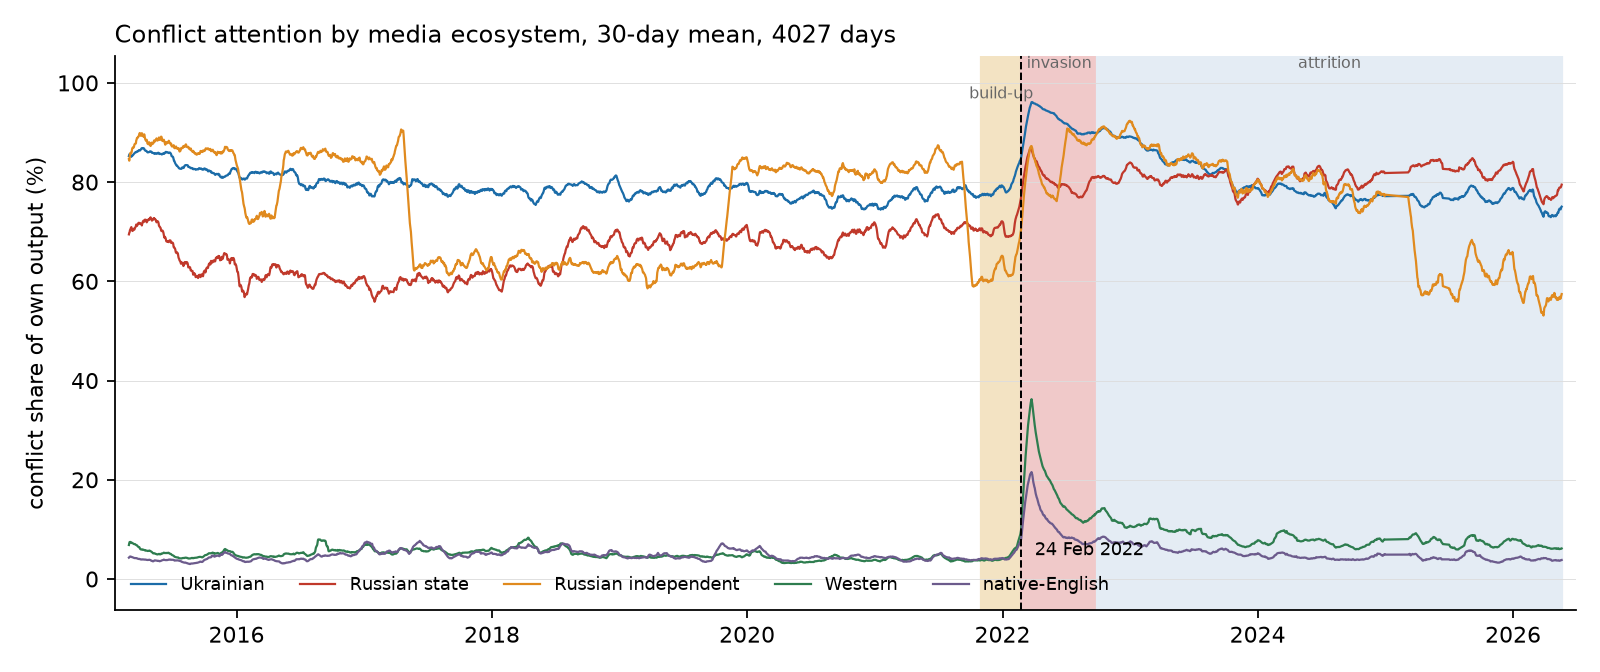
\includegraphics[width=\textwidth]{outputs/figures/fig1_attention_full_sample.png}
\caption{Conflict coverage as a share of each ecosystem's own daily output, 2015--2026, thirty-day moving average. The dashed vertical line marks 24 February 2022 (invasion onset). Shading marks the build-up, invasion and attrition regimes. Ukrainian and Russian series occupy a band of 55--95\% throughout; Western and native-English series remain below 10\% until the invasion.}
\label{fig:attention}
\end{figure}

\begin{figure}[H]
\centering
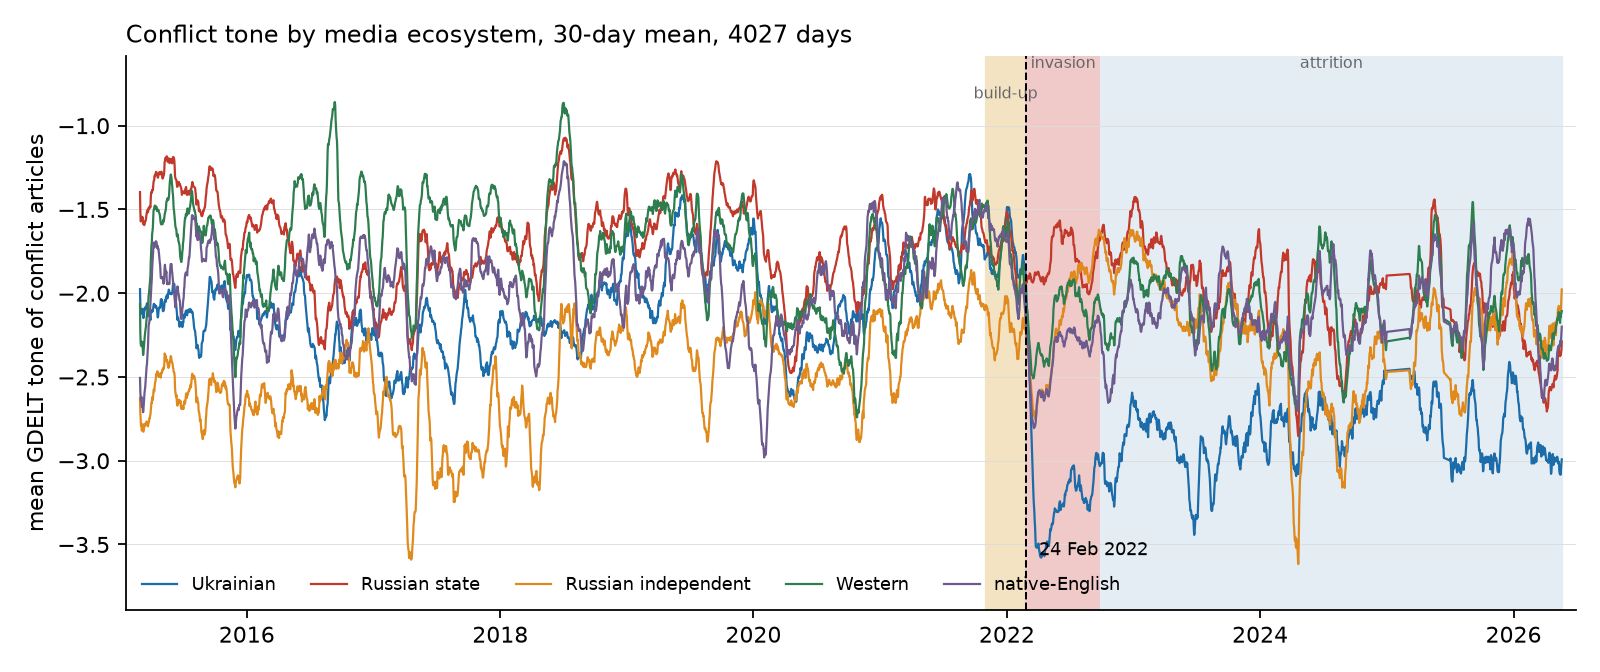
\includegraphics[width=\textwidth]{outputs/figures/fig2_tone_full_sample.png}
\caption{Mean GDELT tone of each ecosystem's conflict articles, same window and smoothing. More negative values indicate more negative coverage. Before 2022 the five tone series interleave with no stable ordering. After 24 February 2022 the Ukrainian line separates downward and stays separated; the Russian state line does not move.}
\label{fig:tone}
\end{figure}

Three features of Figure~\ref{fig:attention} carry descriptive weight. The ecosystems occupy two entirely separate bands across the full eleven years: Ukrainian and Russian series stay between roughly 55\% and 95\%, while Western and native-English series stay below 10\% until 2022. The invasion is visible in only one of those bands --- the Western and native-English lines spike sharply, while the local lines barely can, because they were already near their ceiling. And the spike is temporary where the shift is not: Western attention decays back toward its pre-war level within about two years, while Russian state coverage settles above its pre-war band and stays there.

\subsection{The tone response around the invasion}

Table~\ref{tab:tone_invasion} compares mean conflict tone in the pre-invasion build-up (1 November 2021 -- 23 February 2022) with the first one hundred days after the invasion (24 February -- 5 June 2022).

\begin{table}[H]
\centering
\caption{Conflict tone before and after the full-scale invasion}
\label{tab:tone_invasion}
\begin{threeparttable}
\begin{tabular}{lrrr}
\toprule
Ecosystem & Pre-invasion & Post-invasion & Shift \\
\midrule
Ukrainian (UA) & $-1.77$ & $-3.43$ & $\mathbf{-1.66}$ \\
Native-English (EN\_GLOBAL) & $-1.87$ & $-2.51$ & $-0.64$ \\
Western (WEST) & $-1.88$ & $-2.25$ & $-0.38$ \\
Russian independent (RU\_INDEP) & $-2.23$ & $-2.49$ & $-0.26$ \\
\textbf{Russian state (RU\_STATE)} & $\mathbf{-1.81}$ & $\mathbf{-1.79}$ & $\mathbf{+0.02}$ \\
\bottomrule
\end{tabular}
\begin{tablenotes}
\small
\item Notes: Tone is the mean GDELT tone score for conflict articles in the ecosystem. More negative values indicate more negative language. Pre-invasion: 1 November 2021 -- 23 February 2022. Post-invasion: 24 February -- 5 June 2022. The Russian state result ($+0.02$) is repeated on a fixed panel of 24 state outlets present on both sides of the invasion with at least 200 conflict articles each: the fixed-panel shift is $-0.05$, confirming the aggregate is not an artefact of composition.
\end{tablenotes}
\end{threeparttable}
\end{table}

\textbf{Russian state media's tone did not move when Russia invaded Ukraine.} Every other ecosystem's did, Ukraine's by more than a point and a half. The result is robust to a fixed-outlet restriction: on 24 state outlets present throughout, the shift is $-0.05$. Against Ukrainian media's $-1.66$, that contrast is the order-of-magnitude difference the press-freedom control of \citet{bondarenko2024} would predict.

\subsection{Correlations and structural breaks}

Cross-ecosystem pairwise correlations of daily attention-share changes are low. The maximum pairwise correlation in the full sample is $0.673$ (WEST/EN\_GLOBAL, which overlap by construction); the UA--EN\_GLOBAL correlation is $\mathbf{0.05}$, and the RU\_STATE--EN\_GLOBAL correlation is $0.05$. The ecosystems are distinct populations rather than one population with noise added, which validates using them in a conditional test.

The perception indices also validate externally. WEST and EN\_GLOBAL correlate $0.866$ and $0.884$ in levels with the published Caldara--Iacoviello GPR index in the Ukraine-driven window (2022 onward), and $0.083$ and $0.048$ in the 2017--2019 period when GPR is driven by Korea and Iran. The index tracks the correct conflict when it is Ukraine-relevant and detaches otherwise.

Formal Chow tests at 24 February 2022 and supremum-Wald tests for unknown break dates confirm that attention and tone series break at or near the invasion date in every ecosystem, and that the index-return relationship is structurally stable within the attrition regime.

%=============================================================
\section{Empirical Results}
\label{sec:results}
%=============================================================

\subsection{The test design}
\label{sec:testdesign}

All results are organised around one test, run at increasing sample depth and on increasing demands. The specification is:
\begin{equation}
r_{t+h} = \alpha + \beta_{\text{West}} \mathbf{X}^{\text{West}}_t + \beta_{\text{Local}} \mathbf{X}^{\text{Local}}_t + \gamma Z_t + \varepsilon_{t+h},
\end{equation}
where $r_{t+h}$ is the defence-equity return over horizon $h$, $\mathbf{X}^{\text{West}}_t$ contains attention-share and tone shocks for the Western and native-English ecosystems, $\mathbf{X}^{\text{Local}}_t$ contains the same for the Ukrainian, Russian state, and Russian independent ecosystems, and $Z_t$ contains the regional equity-market control and VIX, both lagged. The object of interest is the \textbf{joint F-test on the three local blocks} conditional on the Western blocks already in the regression. Standard errors are HAC(5) throughout.

The grid runs across daily and weekly frequency, six anticipation episode windows plus the full sample, and five targets: WAERLST, BSHIELDT, ITA, and two hand-built baskets. This produces 31 cells that survive the minimum-observation filter. Benjamini--Hochberg (BH) correction is applied across the whole grid. The pass rule requires BH survivors in at least two independent episode windows with the same sign, or (in Gate 2) in at least one Bloomberg target.

The \textbf{positive control} in every gate is the joint F-test on the Western block in exactly the same cells. The apparatus is informative only if it can find the Western block. It does.

\subsection{Gate 2 --- attention and tone}
\label{sec:gate2}

\begin{table}[H]
\centering
\caption{Gate 2 results: attention share and tone (local versus Western)}
\label{tab:gate2}
\begin{threeparttable}
\begin{tabular}{lrrrl}
\toprule
Specification & Cells & Nominal 5\% & Survive BH & Verdict \\
\midrule
\multicolumn{5}{l}{\textit{Local block (UA + RU\_STATE + RU\_INDEP)}} \\
Same-day alignment & 31 & 8 & 3 & \textbf{FAIL} \\
\textbf{News lagged 1 day (primary)} & \textbf{31} & \textbf{7} & \textbf{0} & \textbf{FAIL} \\
\addlinespace
\multicolumn{5}{l}{\textit{Western block (positive control)}} \\
Same-day alignment & 31 & --- & 3 & PASS \\
News lagged 1 day & 31 & --- & 0 & --- \\
\bottomrule
\end{tabular}
\begin{tablenotes}
\small
\item Notes: 31 cells survive the minimum-observation filter across frequency (daily/weekly), episode window, and target. Benjamini--Hochberg correction at 5\% FDR applied across the whole grid. The primary specification lags news one day, which is the correct alignment given that European markets close at approximately 16:30 UTC while GDELT days are full UTC days. The three same-day BH survivors all fall in a single thin window (2025--26, 60 observations, 13 parameters) and dissolve when the episode is de-crowded by dropping tone. A result confined to one thin corner of a grid is a noise artefact, not a small true effect requiring more power.
\end{tablenotes}
\end{threeparttable}
\end{table}

Under the primary specification --- news lagged one day, which is the defensible alignment --- the local block returns \textbf{zero BH survivors} in 31 cells. The Western block in the same-day arm is detected in 3 of 31 cells at minimum p = 0.0117, confirming the apparatus has power. The three nominal local survivors that appear in the same-day arm are weekly, confined to a single 60-observation window, and dissolve under a reduced parameterisation. The build-up and invasion cells --- the window where any local-information advantage should be at its maximum --- return local p-values from 0.090 to 0.619, nothing close to correction.

\subsection{Gate 3 --- the anticipation structure}
\label{sec:gate3}

Gate 2 tests volume and sentiment. The obvious objection is that neither is the right functional form: what should be priced is not how \textit{much} local media cover the conflict but whether they cover it as something \textit{coming} or something that \textit{has happened}. Gate 3 replaces the raw attention share with the threat/act split described in Section~\ref{sec:measurement} and was pre-registered: the verdict rule, the two arms, the excluded targets and the sign condition were fixed in writing before the test was built.

\begin{table}[H]
\centering
\caption{Gate 3 results: threat/act split, pre-registered (full 4,027-day corpus)}
\label{tab:gate3}
\begin{threeparttable}
\begin{tabular}{lrrrl}
\toprule
Specification & Cells & Nominal 5\% & Survive BH & Verdict \\
\midrule
\multicolumn{5}{l}{\textit{Local block}} \\
\textbf{Primary (news lagged 1 day)} & \textbf{31} & \textbf{9} & \textbf{2} & \textbf{FAIL} \\
Secondary (same-day) & 31 & 3 & 0 & \textbf{FAIL} \\
\addlinespace
\multicolumn{5}{l}{\textit{Western block (positive control)}} \\
Primary (news lagged 1 day) & 31 & --- & 2 & PASS \\
\bottomrule
\end{tabular}
\begin{tablenotes}
\small
\item Notes: Run on the full 4,027-day corpus (2,754 observations in the pooled daily cell). The two primary BH survivors are weekly, both in the 2025--26 episode window, resting on 58 observations with 13 parameters. The pooled daily cell with the most data returns p = 0.10. Under the pre-registered pass rule, neither arm clears: Arm 1 requires a survivor in the Russia window on a Bloomberg target, but the only Russia-window survivor is a hand-built basket explicitly excluded from that arm; Arm 2 requires survivors in two independent windows with the same sign, but Russia daily has the opposite sign to all six weekly cells. Western block detected in 2 of 31 cells, minimum p = 0.0002.
\end{tablenotes}
\end{threeparttable}
\end{table}

The two surviving cells' sign structure is worth reporting precisely because it is seductive. Weekly cells showed a coherent ``buy the rumour, sell the fact'' pattern in Ukrainian media: a shift toward anticipation raised defence returns, a shift toward realisation lowered them. Those four signs were written down and tested on the 2017--19 window, which had not been ingested when the hypothesis was formed. \textbf{7 of 12 signs match; binomial p = 0.387.} Indistinguishable from coin-flips. The pattern was in-sample noise.

\subsection{Gate 4 --- European natural gas}
\label{sec:gate4}

Two nulls on defence equities invite one serious objection: perhaps defence equities are simply a weak testbed, and the link from a Russian newspaper to a U.S. defence contractor's share price is too long to trace. European natural gas has no such excuse. Russia supplied roughly 40\% of EU gas; the Dutch TTF benchmark moved from approximately \euro20 to over \euro300; and Russian state media is the channel through which supply intent was signalled. The test was pre-registered with four conditions; data were ingested only \textit{after} the pre-registration was written.

\begin{table}[H]
\centering
\caption{Gate 4 results: local block on European TTF natural gas}
\label{tab:gate4}
\begin{threeparttable}
\begin{tabular}{lrrr}
\toprule
Window & $n$ & $p$ (local block) & $p$ (Western block) \\
\midrule
(a) Build-up and invasion, 2021-06 -- 2022-06 & 222 & 0.100 & \textbf{0.001} \\
(b) Shutdown and aftermath, 2022-06 -- 2023-06 & 231 & 0.573 & 0.197 \\
(c) Full crisis, 2021-06 -- 2023-12 & 563 & 0.352 & 0.081 \\
\bottomrule
\end{tabular}
\begin{tablenotes}
\small
\item Notes: All four pre-registered conditions fail. No BH survivor in either required window. Window (b) placebos show local-block p-values near 0.10 for Brent ($0.041$), consumer-staples equities ($0.084$) and U.S. natural gas ($0.095$), indicating a common factor rather than a supply channel. The build-up p-value of 0.100 degrades to 0.322 when the ten largest TTF moves are excluded. Russian \textit{independent} media lead the local block in two of four cells, inverting the supply-signalling mechanism that requires \textit{state} media to lead. The exploratory result that motivated this gate was p = 0.0005 on 81 build-up days; the pre-registered confirmatory run on 222 days of the same window returns 0.100.
\end{tablenotes}
\end{threeparttable}
\end{table}

\subsection{Gate 5 --- realised escalation, no price involved}
\label{sec:gate5}

The last objection is that markets may simply fail to impound local information. Gate 5 removes prices from the test altogether and asks whether local perception predicts \textit{realised geopolitical escalation} --- changes in the published Caldara--Iacoviello act component --- one and five days ahead. It too was pre-registered, and data were ingested afterwards.

On \textbf{651 held-out days} never used in any in-sample analysis, the local block returns \textbf{p = 0.16} at $h = 1$ and \textbf{p = 0.30} at $h = 5$. It does not survive twelve lags of the outcome's own dynamics ($p = 0.143$ and $0.566$). The shuffle placebo passes ($0.557$ and $0.799$), confirming the design is not manufacturing significance. The Western block is detected at $p = 0.006$ and $p = 0.041$ in two cells --- the apparatus can see what is there; it does not see the local block because the local block is not there.

\subsection{Out-of-sample return predictability}
\label{sec:efficiency}

Sections~\ref{sec:gate2}--\ref{sec:gate5} test whether local perception is contemporaneously associated with prices. A complementary question is whether it is usable out of sample --- whether an investor could have exploited it. The design follows an expanding-window one-day-ahead forecasting framework with a minimum training window of 250 days and re-estimation at every step. The benchmark is the historical mean. The competing model is the benchmark plus one perception predictor (lagged daily change). The grid has five targets and ten predictors (attention share and tone for each of the five main ecosystems), giving \textbf{50 specifications}. The Clark--West (2007) test arbitrates the nested comparison; Diebold--Mariano with the Harvey--Leybourne--Newbold correction is retained for non-nested comparisons.

\begin{table}[H]
\centering
\caption{Out-of-sample return predictability: Clark--West results across 50 specifications}
\label{tab:efficiency}
\begin{threeparttable}
\begin{tabular}{lrrrr}
\toprule
Quantity & Value \\
\midrule
Specifications & 50 \\
Out-of-sample days & 1,855 \\
Positive Campbell--Thompson R$^2_{\text{OS}}$ & 3 \\
Best R$^2_{\text{OS}}$ & $+0.0011$ (0.11\%) \\
Clark--West $p < 0.05$ & \textbf{0} (2.5 expected by chance) \\
Survive Benjamini--Hochberg at 5\% FDR & \textbf{0} \\
\bottomrule
\end{tabular}
\begin{tablenotes}
\small
\item Notes: Expanding-window one-day-ahead forecasts. Benchmark is the historical mean return. Competing model adds one perception predictor (lagged daily change) per specification. Clark--West (2007) test with Bartlett long-run variance estimator. The zero-rejection count is against 2.5 expected by chance under the null across 50 tests at the 5\% level. Romano--Wolf familywise correction has nothing to correct with zero nominal rejections.
\end{tablenotes}
\end{threeparttable}
\end{table}

\paragraph{Power.} A null result is only a finding if the test that produced it could have found something. Power is established by simulation on the actual return series: a predictor is implanted that explains a known fraction of return variance, returns are regenerated, the identical expanding-window machinery is run, and rejections at the 5\% level are counted.

\begin{table}[H]
\centering
\caption{Simulated power of the Clark--West test (1,855 out-of-sample days)}
\label{tab:power}
\begin{threeparttable}
\begin{tabular}{lrrrrrr}
\toprule
True R$^2_{\text{OS}}$ & 0.0\% & 0.2\% & 0.5\% & 1.0\% & 2.0\% & 4.0\% \\
\midrule
Rejection rate & 0.02 & 0.43 & \textbf{0.82} & 0.98 & 1.00 & 1.00 \\
\bottomrule
\end{tabular}
\begin{tablenotes}
\small
\item Notes: Rejection rate is the fraction of simulations in which the Clark--West test rejects at the 5\% level. Nominal size under the null (first column) is 2\%, confirming the test is conservative rather than liberal. The range of out-of-sample R$^2$ that the predictability literature treats as economically meaningful (roughly 0.5\% to 1.0\%) is detectable at 82\%--98\% power. Zero rejections in 50 specifications is therefore not an artefact of low power; it is a bound.
\end{tablenotes}
\end{threeparttable}
\end{table}

The range of out-of-sample R$^2$ this literature treats as economically meaningful --- roughly 0.5\% to 1.0\% --- is detectable at 82\% to 98\% power with 1,855 out-of-sample days. \textbf{That range is ruled out.} The best observed value (0.11\%) sits below even the 43\%-power threshold, and zero of fifty Clark--West tests reject.

%=============================================================
\section{Robustness: Five Results That Did Not Survive}
\label{sec:robustness}
%=============================================================

Five times in this project a plausible positive appeared, was significant at conventional levels, had a mechanism that could be stated in a sentence, and survived at least one robustness check. None is reported as a finding. Each was retracted and is documented here because the thesis's central result is a null, and a null is worth reporting only if the reader can be shown the search was serious.

\subsection{The omitted market control}
\label{sec:retraction1}

\textbf{What was found.} European defence returns regressed on Caldara--Iacoviello threat shocks showed p = 0.0001 in the build-up window, strengthened monotonically as the window tightened, and survived placebo tests. A related earlier result --- European defence volatility loading on threat at p $< 0.001$ --- falls to the same problem.

\textbf{What killed it.} The market control was the S\&P 500. European defence equities require a European benchmark. Re-running with the STOXX 600:

\begin{table}[H]
\centering
\caption{Build-up window threat shock: SPX versus SXXP control}
\label{tab:control_reversal}
\begin{threeparttable}
\begin{tabular}{lrr}
\toprule
Target & Control = SPX & Control = SXXP \\
\midrule
European defence index & 0.018 & \textbf{0.843} \\
European defence basket & 0.004 & \textbf{0.460} \\
Global A\&D index & 0.002 & \textbf{0.865} \\
U.S. defence basket & 0.009 & \textbf{0.360} \\
\bottomrule
\end{tabular}
\begin{tablenotes}
\small
\item Notes: $p$-values. HAC(5) standard errors. The SPX--SXXP correlation over this window is 0.409, leaving substantial European market variation in the residual when SPX is the control. That residual correlates 0.26 with the threat shock, explaining why the effect is artefactual.
\end{tablenotes}
\end{threeparttable}
\end{table}

\textbf{What survives is better.} Regressing the STOXX 600 itself on the two channels (no market control) gives threat loading of $+0.474$ ($p < 0.0001$), while the same regression on the U.S. market gives nothing. Geopolitical threat is priced market-wide in Europe, not differentially in defence. The retraction turns a fragile sector claim into a robust market result.

\subsection{The truncated sample}

\textbf{What was found.} Gate 3 on a partial ingest of 694 days (the Russia window plus 2025--26) returned 7 BH survivors and a verdict of PASS. The protocol had been written down before the test was built.

\textbf{What killed it.} The ingest was still running. Adding the held-out 2017--19 window --- same grid, same statistic, same correction, nothing changed but the number of days available --- took seven survivors to two and PASS to FAIL. \textbf{A pre-registered test run on a truncated sample is not a pre-registered test.}

\subsection{The register error: \texttt{dw.com}}

\textbf{What was found.} Contrasting Russian state against Russian independent media across the invasion produced a tone wedge that widened materially, with the independent sector's tone falling while the state sector's did not move.

\textbf{What killed it.} \texttt{dw.com} --- Deutsche Welle, the German public broadcaster --- sat in the hand-curated register as a Russian independent outlet. By the criterion this project exists to apply (publisher, not language), it is a Western outlet. It was the ecosystem's largest contributor by volume. Removing it: six outlets, $-0.31$ shift, $p = 0.151$ before the fix; five outlets, $-0.22$, $p = 0.323$ after. The state-versus-independent wedge is not significant and is not claimed. The state-versus-Ukraine contrast ($-1.66$) is robust and is the claim the thesis makes.

\subsection{The small sample: gas}

\textbf{What was found.} On 81 days of the build-up window, the local block explained TTF gas at $p = 0.0005$. The pre-registered confirmatory run on 222 days of the same period returns $p = 0.100$.

\subsection{The in-sample split: escalation}

\textbf{What was found.} The local block predicted realised escalation in both halves of the in-sample period independently --- $p = 0.039$ and $0.024$ in 2017--2021, $p = 0.0001$ and $0.0000$ in 2022--2026. \textbf{What killed it.} On 651 held-out days, $p = 0.16$ and $0.30$. Split-half replication inside a sample is not out-of-sample replication.

%=============================================================
\section{Conclusion}
%=============================================================

This thesis asked whose perception of geopolitical risk is priced in Western defence equities. The answer is the Western narrative's. Conditional on Western and native-English perception, the local ecosystems --- Ukrainian, Russian state, Russian independent --- add no explanatory power to defence-equity returns, in attention, in tone, or in the threat/act anticipation structure. The null holds on European natural gas and on realised escalation itself, each against a positive control that passes. Across 50 out-of-sample specifications the Clark--West test rejects zero times in fifty; simulation shows this design rules out the range of out-of-sample R$^2$ the predictability literature treats as economically meaningful.

\subsection{The mirror of Bondarenko et al.\ (2024)}

The design is a deliberate mirror. \citet{bondarenko2024} find that for the Russian domestic economy the local narrative dominates and the English-language one is redundant. Running the same contrast on the counterparty's assets produces the reverse asymmetry. Neither result generalises into ``local media matter'' or ``local media do not''; taken together they say something more specific: each market prices the information ecosystem it inhabits. Russian economic agents respond to Russian-language risk perception; Western defence-equity investors respond to Western risk perception, and eleven years of what Ukrainian and Russian outlets published about their own war contributes nothing measurable on top.

\subsection{The methodological contribution}

Five pre-registered or control-based tests, five retractions, with the sequence documented rather than buried, is a more useful result for anyone doing this kind of work than a sixth test would have been. The five failure modes are all different: two omitted-variable problems, one truncated sample, one small sample, and one in-sample split that did not generalise. That is not one mistake repeated; it is five distinct ways for a media-and-markets study to produce a convincing artefact.

\subsection{Limitations and extensions}

First, the analysis does not identify causal effects; the design is associational, and prices and narratives respond to the same underlying events. Second, the daily frequency may be too coarse for some reactions; intraday data would allow a cleaner analysis of price discovery around specific announcements. Third, GDELT tone and source classification contain measurement error. Fourth, the firm-level cross-section --- which would allow testing whether defence-revenue exposure scales the response --- is not available; SIPRI constituent data were not obtained for this project. Future work could apply multilingual transformer models directly to article text, compare this conflict with others, and extend the asset-class coverage to bond markets and currencies.

\newpage
\bibliography{references}

\end{document}
